% !Mode::"TeX:UTF-8"

% -------------------- Information --------------------

\newcommand{\TITLE}{常微分方程初值问题}
\newcommand{\AUTHOR}{Jason}
\newcommand{\SUBJECT}{偏微分方程数值解}
\newcommand{\KEYWORDS}{}

% -------------------- Packages --------------------

\documentclass[a4paper, 12pt]{ctexart}
\usepackage{amsmath}
\usepackage{amssymb}
% \usepackage{amsthm} % 定理格式 由ntheorem代替.
\usepackage{authblk} % 作者 (见校赛论文).
\usepackage{array}
\usepackage{bigfoot} % to allow verbatim in footnote.
\usepackage{bm} % \bm for bold symbols.
\usepackage{boldline} % 长表格表格线加粗.
\usepackage{caption} % 题注.
\usepackage{commath} % abs, norm
\usepackage{enumerate}
% \usepackage{enumitem} 用enumerate包代替.
\usepackage{fancyhdr} % 脚注.
\usepackage{filecontents}
\usepackage{flafter} % 不让float出现在定义之前的地方.
\usepackage{float} % 你们这帮float给我乖乖听话 HHHHHHHHHHH.
\usepackage[T1]{fontenc} % Bera Mono Font
\usepackage{fontspec} % 字体.
\usepackage{graphicx}
\usepackage{hyperref}
\usepackage{lastpage}
\usepackage{letltxmacro} % \let
\usepackage{lipsum}
\usepackage{listings} % 排版程序语言.
\usepackage{longtable} % 长表格.
\usepackage{makecell} % 表格线加粗 \Xhline{1.2pt}.
\usepackage{mathtools} % \xleftrightarrow.
\usepackage{mathrsfs} % \mathscr
\usepackage{multirow} % 合并单元格.
\usepackage[square, numbers, sort&compress]{natbib} % 引用.
\usepackage[thmmarks, amsmath, thref]{ntheorem} % 定理格式.
\usepackage[section]{placeins} % 使图像不会显示在别的部分 若过于严格则换成[below].
\usepackage{stackrel} % 上下写 见校赛论文.
\usepackage{subcaption} % subcaption and subfigure
% \usepackage{SUBSubsubsection}
\usepackage{titlesec} % Section标题格式.
\usepackage{varioref} % For Cross References.
\usepackage[dvipsnames]{xcolor} % 颜色声明.
\usepackage{xfrac} %\sfrac{}{}
\usepackage[all, cmtip]{xy} % Commutive diagram.

% Require `ntheorem'

\usepackage[mathlines, edtable]{lineno} % Line numbers.
    %\begin{edtable}{tabular}[<args>] <entries> \end{edtable}

% Require `xcolor'

\usepackage[numbered, framed]{matlab-prettifier}
\usepackage{pgfplots}
\usepackage{pgfplotstable}
\usepackage{tikz}

% Incompatible with `matlab-prettifier'

\usepackage[printwatermark]{xwatermark} % Foreground Watermarks.

% -------------------- Settings --------------------

% Title

\title{\TITLE}
\author{\AUTHOR}
\date{\today}

% Package: caption

\captionsetup{
    margin    =   6pt,
    font      =   small,
    labelfont =   bf
}

% Package: ctex

\setCJKfamilyfont{fzstk}{FZShuTi} % 方正舒体
\newcommand{\fzstk}{\CJKfamily{fzstk}}

% Package: fancyhdr

\setlength{\headheight}{15pt}
\lhead{Copyright \copyright\ \AUTHOR}
\rhead{Page \thepage\ of \pageref{LastPage}}

% Package: graphicx

\graphicspath{{resources/}} % 图像文件目录

% Package: hyperref

\hypersetup{
    linktoc             =   all,
    colorlinks          =   true,
    linkcolor           =   cyan,
    anchorcolor         =   black,
    citecolor           =   green,
    filecolor           =   cyan,
    menucolor           =   red,
    runcolor            =   filecolor,
    urlcolor            =   magenta,
	pdftitle           	=   {\TITLE},
	pdfauthor          	=   {\AUTHOR},
	pdfsubject         	=   {\SUBJECT},
	pdfcreator			=	{Visual Studio Code},
	pdfproducer			=	{XeLaTeX with documentclass ctexart},
	pdfkeywords        	=   {\KEYWORDS},
    bookmarksnumbered   =   true,
    pdfstartview        =   FitH,
    pdfpagelayout       =   OneColumn
}

% Package: lineno

\renewcommand{\linenumberfont}{\normalfont\scriptsize\sffamily}

\let\oldlstinputlisting\lstinputlisting
\renewcommand{\lstinputlisting}[2][\empty]{
    \par\nolinenumbers\oldlstinputlisting[#1]{#2}\linenumbers\par
}

\let\oldlstlisting\lstlisting
\let\oldendlstlisting\endlstlisting
\renewenvironment{lstlisting}
    {\par\nolinenumbers\oldlstlisting}
    {\oldendlstlisting\endnolinenumbers\par}

\let\oldtable\table
\let\oldendtable\endtable
\renewenvironment{table}
    {\par\nolinenumbers\oldtable}
    {\oldendtable\endnolinenumbers\par}

% Package: listings

%% Title

\renewcommand\lstlistingname{代码}
\renewcommand\lstlistlistingname{代码}

%% Lstinline with color box

\LetLtxMacro{\oldlstinline}{\lstinline}
\renewcommand{\lstinline}[2][]{\colorbox{lightgray}{\oldlstinline[#1]{#2}}}
\newcommand{\matlabinline}[1]{
    \lstinline[style=MATLAB-editor, basicstyle=\mlttfamily]{#1}}

\lstset{
    breaklines=true,
    backgroundcolor=\color{lightgray},
    basicstyle=\scriptsize,
    inputpath=resources/,
    numbers=left,
    numberstyle={\color{black!33}\scriptsize\sffamily},
    xleftmargin=2em,
    xrightmargin=2em
}

% Package: ntheorem

%% Theorem
\newtheorem{theorem}{Theorem}[section]
\newtheorem{lemma}[theorem]{Lemma}
\newtheorem{corollary}[theorem]{Corollary}
%% Problem
\theoremstyle{plain}
\newtheorem{problem}{Problem}[section]
%% Proposition
\newtheorem{proposition}{Proposition}[section]
%% Conjecture
\newtheorem{conjecture}[proposition]{Conjecture}
%% Definition
\theoremstyle{plain}
\theoremheaderfont{\bfseries}
\theorembodyfont{\rmfamily}
\newtheorem{definition}{Definition}[section]
%% Note
\theoremstyle{plain}
\theoremheaderfont{\itshape}
\theorembodyfont{\itshape}
\newtheorem{note}{Note}[section]
%% Proof
\theoremstyle{nonumberplain}
\theoremheaderfont{\itshape}
\theorembodyfont{\upshape}
\theoremseparator{.}
\theoremsymbol{\ensuremath{\square}}
\newtheorem{proof}{Proof}
%% Solution
\theoremsymbol{\ensuremath{\blacksquare}}
\newtheorem{solution}{Solution}

% Package: pgfplots

\pgfplotsset{width=7cm, compat=1.16}

% Package: pgfplotstable

\pgfplotstableset{
    every head row/.style={before row=\Xhline{1.2pt},after row=\hline},
    every last row/.style={after row=\Xhline{1.2pt}}
}

% Package: varioref

\renewcommand{\reftextbefore}
    {on the \reftextvario{preceding page}{page before}}
\renewcommand{\reftextafter}
    {on the \reftextvario{following}{next} page}
\renewcommand{\reftextfacebefore}
    {on the \reftextvario{facing}{preceding} page}
\renewcommand{\reftextfaceafter}
    {on the \reftextvario{facing}{next} page}
\renewcommand{\reftextfaraway}[1]
    {on page \pageref{#1}}

%% Label formats

\labelformat{lstlisting}{代码#1}
\labelformat{equation}{式(#1)}
\labelformat{figure}{图#1}
\labelformat{table}{表#1}
\labelformat{problem}{Problem #1}

% Package: xwatermark

\newsavebox\mybox
\savebox\mybox{\tikz[color=cyan, opacity=0.2]\node{\fzstk\SUBJECT};}
\newwatermark*[
    allpages,
    angle=45,
    scale=6,
    xpos=-20,
    ypos=15
]{\usebox\mybox}

% -------------------- General new commands --------------------

\DeclareMathAlphabet{\mathsfsl}{OT1}{cmss}{m}{sl}

\DeclareMathOperator{\arcosh}{arcosh}
\DeclareMathOperator{\Arcosh}{Arcosh}
\DeclareMathOperator*{\Beta}{B}
\DeclareMathOperator{\Log}{Log}
\DeclareMathOperator*{\real}{Re}
\DeclareMathOperator*{\image}{Im}

% Expectation

\newcommand{\expect}{\operatorname{E}\expectarg}
\DeclarePairedDelimiterX{\expectarg}[1]{(}{)}{
    \ifnum\currentgrouptype=16 \else\begingroup\fi
    \activatebar#1
    \ifnum\currentgrouptype=16 \else\endgroup\fi
}

\newcommand{\innermid}{\nonscript\;\delimsize\vert\nonscript\;}
\newcommand{\activatebar}{
    \begingroup\lccode`\~=`\|
    \lowercase{\endgroup\let~}\innermid
    \mathcode`|=\string"8000
}

\newcommand*{\BC}{\mathbb{C}}
\newcommand*{\BR}{\mathbb{R}}
\newcommand*{\diff}{\mathop{}\!\mathrm{d}}
\newcommand*{\matr}[1]{\ensuremath{\mathsfsl{#1}}} % italic sans serif
\newcommand*{\me}{\mathrm{e}}
\newcommand*{\mi}{\mathrm{i}}
\newcommand*{\restrict}[1]{\raisebox{-.5ex}{$\vert$}_{#1}}
\newcommand*{\vect}[1]{\bm{#1}}

% -------------------- Specific new commands --------------------



% -------------------- Document --------------------

\begin{document}

    % -------------------- Title Page --------------------

    \maketitle
    \thispagestyle{empty}
    \pagenumbering{roman}

    % -------------------- Abstract Page --------------------

    % -------------------- Contents --------------------

    \newpage
    \tableofcontents

    % -------------------- Body --------------------

    \newpage
    \pagestyle{fancy}
    \pagenumbering{arabic}
    \linenumbers

    \section{问题与解答}

    \begin{problem}
        \label{problem: 1}
        考虑一阶常微分方程初值问题:
        \begin{equation}
            \label{equation: problem1}
            \begin{aligned}
                v'(t) &= g - \frac{c_{d}}{m}v^{2},\quad t\in [0, 10],\\
                v(0) &= 0,
            \end{aligned}
        \end{equation}
        其中$g=9.81\mathrm{m/s^{2}}$, $m=68.1\mathrm{kg}$, $c_{d}=0.25\mathrm{kg/m}$.

        \begin{itemize}
            \item 用标准4阶4段龙格-库塔公式求解.
        \end{itemize}
    \end{problem}

    \begin{solution}
        运行脚本\ref{matlab: 1}可得以下图像:
        \begin{figure}[H]
            \centering
            \begin{subfigure}[b]{0.45\textwidth}
                \centering
                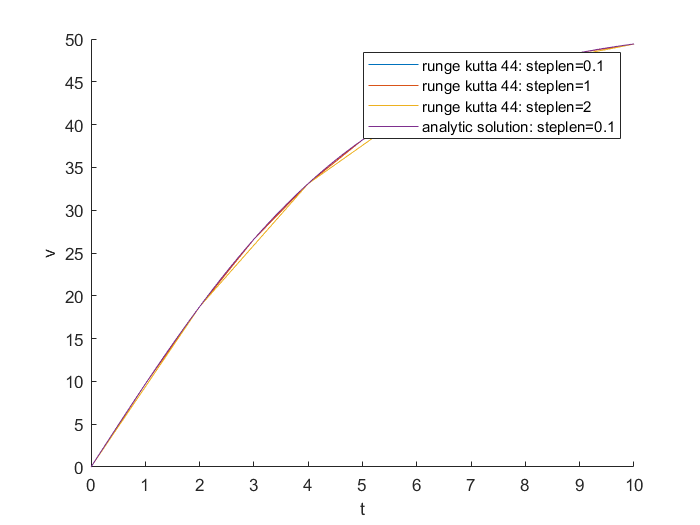
\includegraphics[width=\textwidth]{wc11.png}
                \caption{数值解和解析解}
            \end{subfigure}
            \hfill
            \begin{subfigure}[b]{0.45\textwidth}
                \centering
                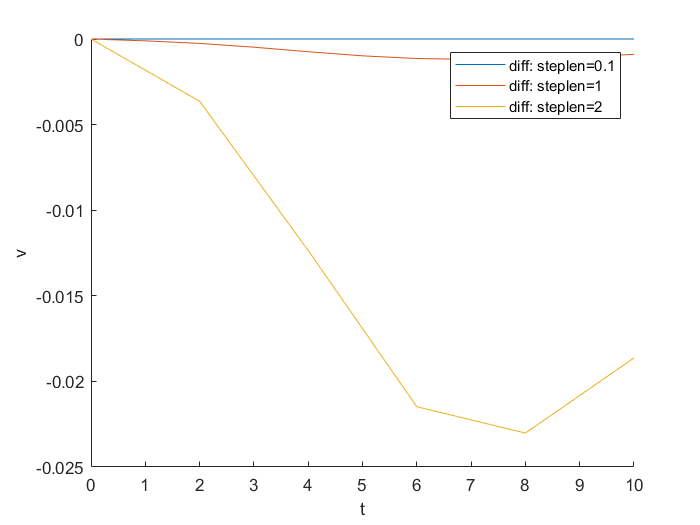
\includegraphics[width=\textwidth]{wc12.png}
                \caption{数值解与解析解之间的差}
            \end{subfigure}
            \caption{\ref{problem: 1}图像}
       \end{figure}
       从图像中可见随着步长的减少, \hyperref[equation: problem1]{原初值问题}的数值解趋向于解析解.
    \end{solution}

    \begin{problem}
        \label{problem: 2}
        考虑一阶常微分方程组初值问题:
        \begin{equation}
            \label{equation: problem2}
            \begin{aligned}
                u'(t) &= au - buv,\\
                v'(t) &= -cv + duv,\quad t\in [0, 30],\\
                u(0) &= 2,\quad v(0) = 1,
            \end{aligned}
        \end{equation}
        其中$a=1.2$, $b=0.6$, $c=0.8$, $d=0.3$.
        \begin{itemize}
            \item 用标准4阶4段龙格-库塔公式求解.
            \item 用Runge-Kutta-Fehlberg算法求解.
        \end{itemize}
    \end{problem}

    \begin{solution}
        运行脚本\ref{matlab: 2}可得以下图像:
        \begin{figure}[H]
            \centering
            \begin{subfigure}[b]{0.45\textwidth}
                \centering
                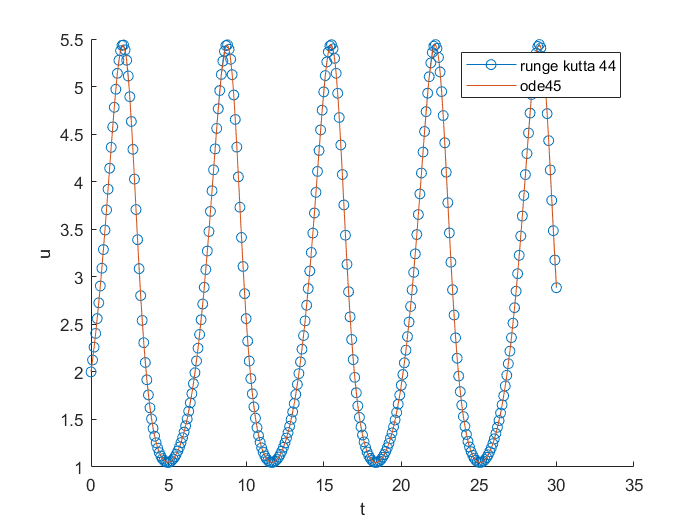
\includegraphics[width=\textwidth]{wc21.png}
                \caption{$u=u(t)$}
            \end{subfigure}
            \hfill
            \begin{subfigure}[b]{0.45\textwidth}
                \centering
                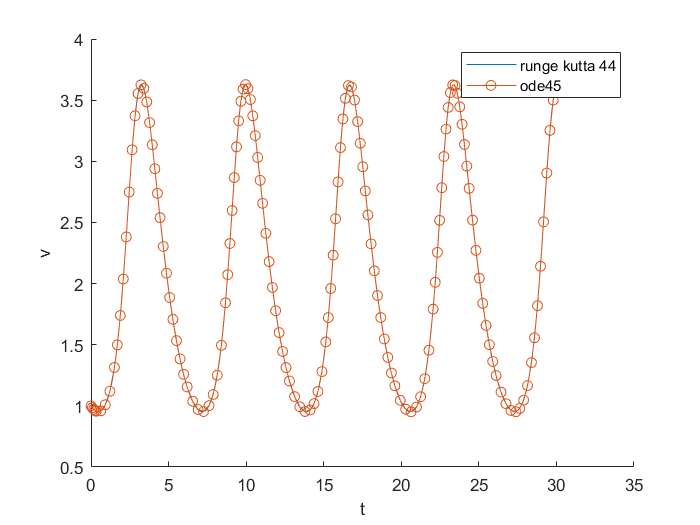
\includegraphics[width=\textwidth]{wc22.png}
                \caption{$v=v(t)$}
            \end{subfigure}
            \caption{\ref{problem: 2}图像}
       \end{figure}
       从图像中我们可以看出用$h=0.1$的标准4阶4段龙格-库塔公式与用Runge-Kutta-Fehlberg算法求出的数值解十分接近. 同时也可以发现Runge-Kutta-Fehlberg算法实际取的点数要少一半左右, 在保证精度的前提下节省了计算量.
    \end{solution}

    \begin{problem}
        \label{problem: 3}
        考虑一阶常微分方程组初值问题:
        \begin{equation}
            \label{equation: problem3}
            \begin{aligned}
                u'(t) &= -au - av,\\
                v'(t) &= -ru - v + uw,\quad t\in [0, 20],\\
                w'(t) &= -bw + uv,\\
                u(0) &= 5,\quad v(0) = 5,\quad w(0) = 5,
            \end{aligned}
        \end{equation}
        其中$a=10$, $b=8/3$, $r=28$.
        \begin{itemize}
            \item 用标准4阶4段龙格-库塔公式求解.
            \item 用Runge-Kutta-Fehlberg算法求解.
        \end{itemize}
    \end{problem}

    \begin{solution}
        运行脚本\ref{matlab: 3}可得以下图像:
        \begin{figure}[H]
            \centering
            \begin{subfigure}[b]{0.3\textwidth}
                \centering
                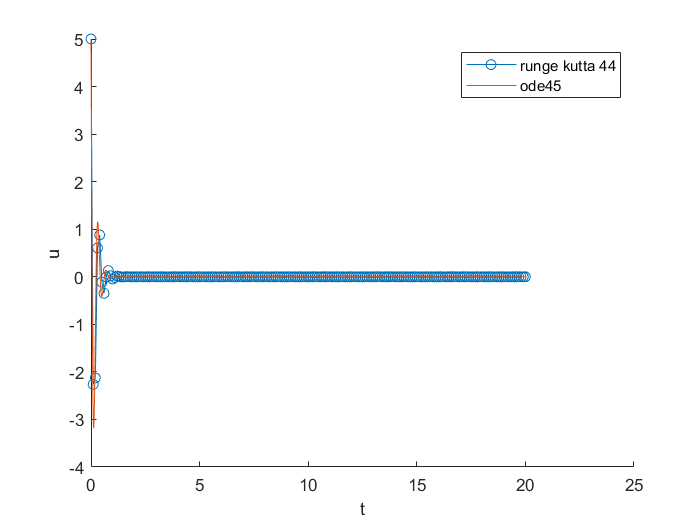
\includegraphics[width=\textwidth]{wc31.png}
                \caption{$u=u(t)$}
            \end{subfigure}
            \hfill
            \begin{subfigure}[b]{0.3\textwidth}
                \centering
                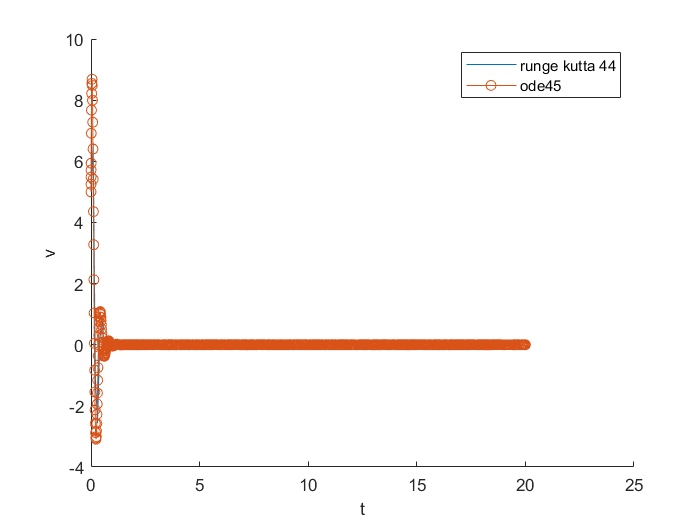
\includegraphics[width=\textwidth]{wc32.png}
                \caption{$v=v(t)$}
            \end{subfigure}
            \begin{subfigure}[b]{0.3\textwidth}
                \centering
                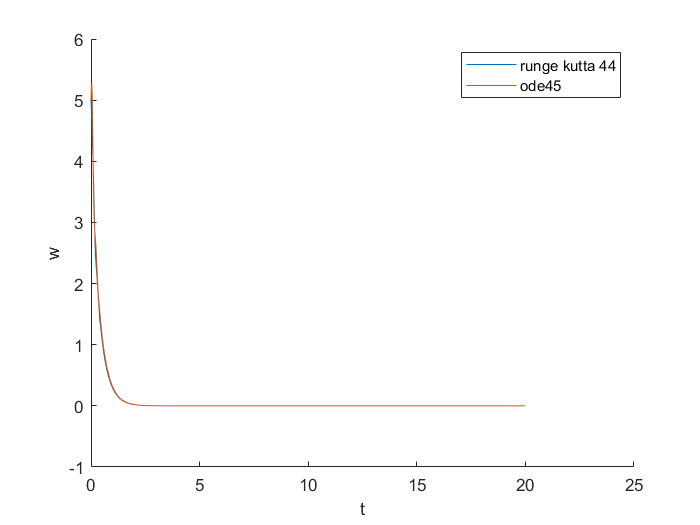
\includegraphics[width=\textwidth]{wc33.png}
                \caption{$w=w(t)$}
            \end{subfigure}
            \caption{\ref{problem: 3}图像}
       \end{figure}
       从中可以发现, 由于在0附近\hyperref[equation: problem3]{原初值问题}的解振荡, 而Runge-Kutta-Fehlberg算法取的点较多, 因此该数值解要更准确一些.
    \end{solution}

    \begin{problem}
        \label{problem: 4}
        考虑一阶常微分方程组初值问题:
        \begin{equation}
            \label{equation: problem4}
            \begin{aligned}
                u'(t) &= v,\\
                v'(t) &= \mu(1-u^{2})v-u,\quad t\in [0, 20],\\
                u(0) &= v(0) = 1,
            \end{aligned}
        \end{equation}
        其中$\mu=1000$.
        \begin{itemize}
            \item 用标准4阶4级龙格-库塔公式求解.
            \item 用Runge-Kutta-Fehlberg算法求解.
        \end{itemize}
    \end{problem}

    \begin{solution}
        运行脚本\ref{matlab: 4}可得以下图像:
        \begin{figure}[H]
            \centering
            \begin{subfigure}[b]{0.45\textwidth}
                \centering
                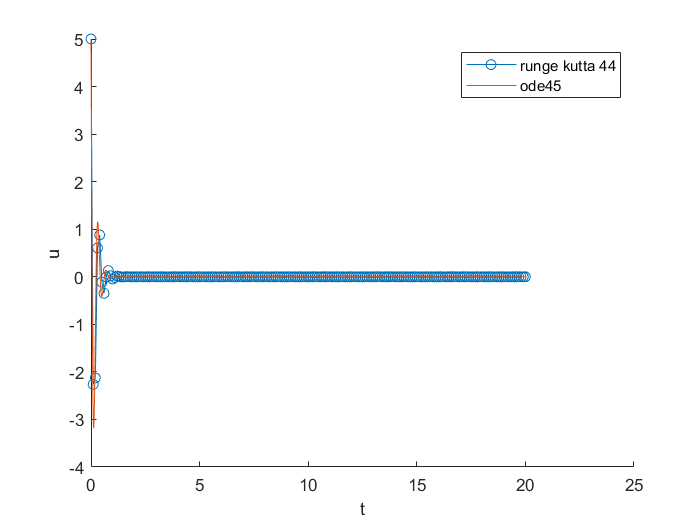
\includegraphics[width=\textwidth]{wc31.png}
                \caption{$u=u(t)$}
            \end{subfigure}
            \hfill
            \begin{subfigure}[b]{0.45\textwidth}
                \centering
                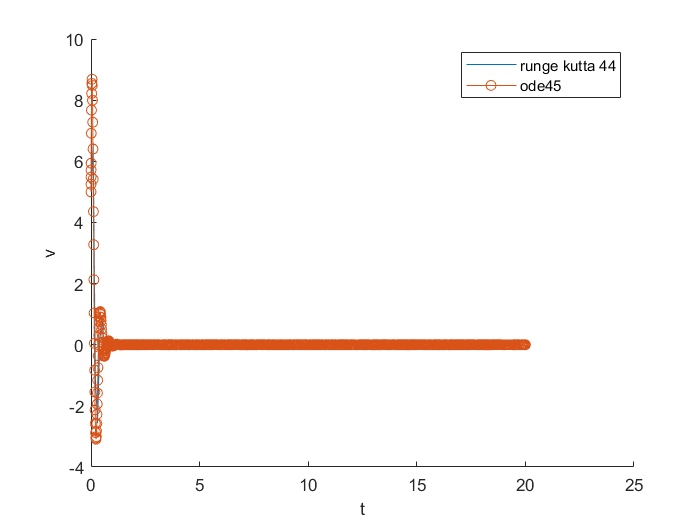
\includegraphics[width=\textwidth]{wc32.png}
                \caption{$v=v(t)$}
            \end{subfigure}
            \caption{\ref{problem: 4}图像}
       \end{figure}
       这里在龙格-库塔公式中我们从大到小尝试了不同的$h$值, 直到$h=0.0001$时算法才收敛, 可见\hyperref[equation: problem4]{原初值问题}刚性程度很高.
    \end{solution}

    \section{比较不同ODE求解函数的计算效果}

    这里我们分别采用$h=0.1$的标准4阶4段龙格-库塔公式和MATLAB内置的ode45, ode23, ode113, ode15s, ode23s, ode23t, ode23tb函数对上述四个初值问题进行求解, 通过绘图和MATLAB的探查器来比较收敛情况与求解速度, 得到以下表格(其中红色表示不收敛或偏差较大):
    \begin{table}[H]
        \begin{center}
            \caption{不同ODE求解函数的计算时间(单位: $\mathrm{s}$)}
            \begin{tabular}{cccccccc}
                \Xhline{1.2pt}
                rk44 & ode45 & ode23 & ode113 & ode15s & ode23s & ode23t & ode23tb\\
                \hline
                0.008 & 0.047 & 0.026 & 0.053 & 0.064 & 0.051 & 0.067 & 0.056\\
                \textcolor{red}{0.015} & 0.047 & 0.035 & 0.074 & 0.098 & 0.065 & 0.091 & 0.074\\
                \textcolor{red}{0.013} & 0.051 & 0.039 & 0.086 & 0.122 & 0.083 & 0.119 & 0.084\\
                \textcolor{red}{0.012} & 0.632 & 0.486 & 1.566 & \textcolor{red}{0.131} & \textcolor{red}{0.079} & 0.112 & 0.087\\
                \Xhline{1.2pt}
            \end{tabular}
        \end{center}
    \end{table}

    当然表中数据会受到电脑实施状态的影响, 具体数值仅供参考. 从中我们还是可以发现针对刚性方程的函数(如ode15s, ode23s, ode23t, ode23tb)在面对刚性或者非刚性方程时求解速度相差不大, 能较高效率的求出刚性方程的近似解, 不过精度不高; 针对非刚性方程的函数(如ode45, ode23, ode113)面对刚性方程时会花费大量时间, 在本次试验的例子中还能给出较为准确的解, 但是不确定面对更为苛刻的刚性方程时表现会如何; 没有自适应步长的标准4阶4段龙格-库塔公式在解的振荡点附近显得比较无力, 必须要将步长减得很小, 但这样的话运算时间就很高了.

    % -------------------- Bibliography --------------------

    % \newpage
    % \bibliography{Principles_of_Mathematical_Analysis}
    % \bibliographystyle{plain}

    % -------------------- Appendix --------------------

    \newpage
    \appendix

    \section{通用函数}

    \subsection{标准4阶4段龙格-库塔公式}

    这里值得注意的是这个函数与ode45函数的输入参数一致, 并且也可求解常微分方程组的初值问题.

    \lstinputlisting[
        caption=ode\_runge\_kutta\_44.m,
        style=MATLAB-editor,
        basicstyle=\mlttfamily\scriptsize
    ]{ode_runge_kutta_44.m}

    \section{求解脚本}

    \subsection{\ref{problem: 1}}

    \lstinputlisting[
        caption=问题一求解脚本: wc1.m,
        label={matlab: 1},
        style=MATLAB-editor,
        basicstyle=\mlttfamily\scriptsize
    ]{wc1.m}

    \subsection{\ref{problem: 2}}

    \lstinputlisting[
        caption=问题二求解脚本: wc2.m,
        label={matlab: 2},
        style=MATLAB-editor,
        basicstyle=\mlttfamily\scriptsize
    ]{wc2.m}

    \subsection{\ref{problem: 3}}

    \lstinputlisting[
        caption=问题三求解脚本: wc3.m,
        label={matlab: 3},
        style=MATLAB-editor,
        basicstyle=\mlttfamily\scriptsize
    ]{wc3.m}

    \subsection{\ref{problem: 4}}

    \lstinputlisting[
        caption=问题四求解脚本: wc4.m,
        label={matlab: 4},
        style=MATLAB-editor,
        basicstyle=\mlttfamily\scriptsize
    ]{wc4.m}

\end{document}
